\chapter{减数分裂、遗传混合与遗传}\label{ch:b2:meiosis-heredity}

双亲皆为褐眼，却生下一个蓝眼孩子，没有人会感到意外；
同一对父母所生的两个孩子从不完全相同，这同样不足为奇。
这两个事实都源于同一过程：每个卵细胞和每个精子形成时，
每种染色体均有两份拷贝的细胞，
恰好将其中一份随机传给配子，
而在此之前，两份拷贝已交换片段。
每一次受精随后，便把两组从未相遇过的半套染色体合在一起。
本章讲述这一过程——\omterm{def:b2:meiosis-heredity:meiosis}{减数分裂}——以及由此而来的遗传规律：
孟德尔比例及其例外情况，
同一染色体上基因的\omterm{def:b2:meiosis-heredity:linkage}{连锁}，以及\omterm{def:b2:meiosis-heredity:linkage}{连锁}所绘制的图谱，
\omterm{prop:b2:meiosis-heredity:sexlinked}{性染色体}的特殊遗传方式，
以及细胞器的特殊遗传方式。

\section{减数分裂}

\begin{definition}[减数分裂]\label{def:b2:meiosis-heredity:meiosis}
\index{减数分裂}\index{单倍体}\index{二倍体}
一个\emph{二倍体}细胞（$2n$）中每种染色体各有两条\emph{同源}
染色体，分别来自父母双方，基因内容相同，但\omterm{def:b2:meiosis-heredity:vocabulary}{等位基因}不一定相同。
\emph{减数分裂}是一对分裂，可使一个二倍体细胞
变为四个\emph{单倍体}细胞，
即每个细胞（$n$）中每种染色体各含一条。分裂前先有一次复制，
使每条染色体以两条姐妹染色单体的形式进入分裂；
第一次分裂分离\emph{同源染色体}（减数），
第二次分裂分离\emph{姐妹染色单体}（等数），与有丝分裂相同。在动物中，
减数分裂产生配子；在植物和真菌中，
它产生孢子（\cref{ch:b2:plant-life-cycles}）；在一切有性生殖的生物中，
它使染色体数目减半，
以便受精时数目再次加倍。
\end{definition}

\begin{proposition}[各阶段]\label{prop:b2:meiosis-heredity:stages}
\index{前期 I}\index{联会}\index{交叉}\index{交叉互换}
\emph{前期 I}历时较长，是混合发生之处。复制后的染色体凝缩，
每条染色体找到其同源染色体，
并与之逐基因配对（\emph{\omterm{prop:b2:meiosis-heredity:stages}{联会}}），由一种蛋白质梯状结构——
\emph{\omterm{prop:b2:meiosis-heredity:stages}{联会}复合体}——维系，形成由四条染色单体组成的\emph{二价体}；
非姐妹染色单体在相应位点断裂并重新连接，
即\emph{\omterm{prop:b2:meiosis-heredity:stages}{交叉互换}}，每个二价体上发生
一次至数次；\omterm{prop:b2:meiosis-heredity:stages}{联会}复合体解体后，同源染色体仅在这些交换位点保持相连，
在显微镜下可见为\emph{\omterm{prop:b2:meiosis-heredity:stages}{交叉}}。
\emph{中期 I}：二价体排列于纺锤体上，每对的取向随机——
母源同源染色体朝向一极或另一极，
与其他各对彼此独立。\emph{后期 I}：
同源染色体分离，姐妹染色单体仍结合在一起，每极
获得 $n$ 条染色体，每条含两条染色单体。\emph{末期 I}
以及通常不再复制的\emph{\omterm{def:b2:meiosis-heredity:meiosis}{减数分裂} II}：$n$ 条染色体逐条排列，
姐妹染色单体分离，形成四个\omterm{def:b2:meiosis-heredity:meiosis}{单倍体}细胞核。\omterm{def:b2:meiosis-heredity:meiosis}{减数分裂} I 历时
从数小时到数十年不等（人类卵母细胞自出生前即停滞于
前期 I，直至排卵）；
\omterm{def:b2:meiosis-heredity:meiosis}{减数分裂} II 仅需一小时。
\end{proposition}

\begin{omfigure}
\begin{tikzpicture}[every node/.style={font=\scriptsize}]
  % helper: cell outline at (x,y)
  \foreach \x/\lab in {0/{前期 I：联会、交叉互换}, 3.2/{中期 I：二价体排列}, 6.4/{后期 I：同源染色体分离}, 9.6/{减数第二次分裂：染色单体分离}}
    { \draw[thick] (\x+1.2,0) circle (1.15); \node[below, align=center, text width=2.8cm] at (\x+1.2,-1.2) {\lab}; }
  % prophase I: one bivalent with chiasma
  \draw[very thick, omDef] (0.8,-0.5) -- (0.8,0.5); \draw[very thick, omDef] (1.0,-0.5) -- (1.0,0.5);
  \draw[very thick, omThm] (1.4,-0.5) -- (1.4,0.5); \draw[very thick, omThm] (1.6,-0.5) -- (1.6,0.5);
  \draw[very thick, omDef] (1.0,0.1) -- (1.4,-0.1); \draw[very thick, omThm] (1.4,0.1) -- (1.0,-0.1);
  \fill[white] (0.9,-0.03) rectangle (1.5,0.03);
  \draw[very thick, omDef] (1.0,0.1) -- (1.4,-0.1); \draw[very thick, omThm] (1.4,0.1) -- (1.0,-0.1);
  \node[omExo!60!black] at (1.2,-0.85) {交叉};
  % metaphase I: two bivalents on the plate, spindle
  \begin{scope}[xshift=3.2cm]
    \draw[gray, dashed] (1.2,-1.0) -- (1.2,1.0);
    \foreach \y in {0.45,-0.45} {
      \draw[very thick, omDef] (0.95,\y-0.25) -- (0.95,\y+0.25); \draw[very thick, omDef] (1.08,\y-0.25) -- (1.08,\y+0.25);
      \draw[very thick, omThm] (1.32,\y-0.25) -- (1.32,\y+0.25); \draw[very thick, omThm] (1.45,\y-0.25) -- (1.45,\y+0.25);
    }
    \draw[gray] (0.15,0) -- (0.95,0.45); \draw[gray] (0.15,0) -- (0.95,-0.45);
    \draw[gray] (2.25,0) -- (1.45,0.45); \draw[gray] (2.25,0) -- (1.45,-0.45);
  \end{scope}
  % anaphase I
  \begin{scope}[xshift=6.4cm]
    \foreach \y in {0.45,-0.45} {
      \draw[very thick, omDef] (0.45,\y-0.25) -- (0.45,\y+0.25); \draw[very thick, omDef] (0.58,\y-0.25) -- (0.58,\y+0.25);
      \draw[very thick, omThm] (1.82,\y-0.25) -- (1.82,\y+0.25); \draw[very thick, omThm] (1.95,\y-0.25) -- (1.95,\y+0.25);
    }
    \draw[->, gray] (1.2,0) -- (0.75,0); \draw[->, gray] (1.2,0) -- (1.65,0);
  \end{scope}
  % meiosis II: four cells
  \begin{scope}[xshift=9.6cm]
    \foreach \p/\c in {(0.75,0.5)/omDef,(1.65,0.5)/omDef,(0.75,-0.5)/omThm,(1.65,-0.5)/omThm} {
      \draw[thick, gray!60] \p circle (0.38);
      \draw[very thick, \c] \p ++(-0.12,-0.2) -- ++(0,0.4);
      \draw[very thick, \c] \p ++(0.12,-0.2) -- ++(0,0.4);
    }
  \end{scope}
\end{tikzpicture}

{\small 两对同源染色体的\omterm{def:b2:meiosis-heredity:meiosis}{减数分裂}（母源为蓝色，父源为红色，
每条含两条染色单体）。同源染色体在前期 I 配对并交换片段，
在中期 I 排列为二价体，在后期 I 分离；
\omterm{def:b2:meiosis-heredity:meiosis}{减数分裂} II 使染色单体分开，
形成四个\omterm{def:b2:meiosis-heredity:meiosis}{单倍体}细胞。}
\end{omfigure}

\begin{omfigure}
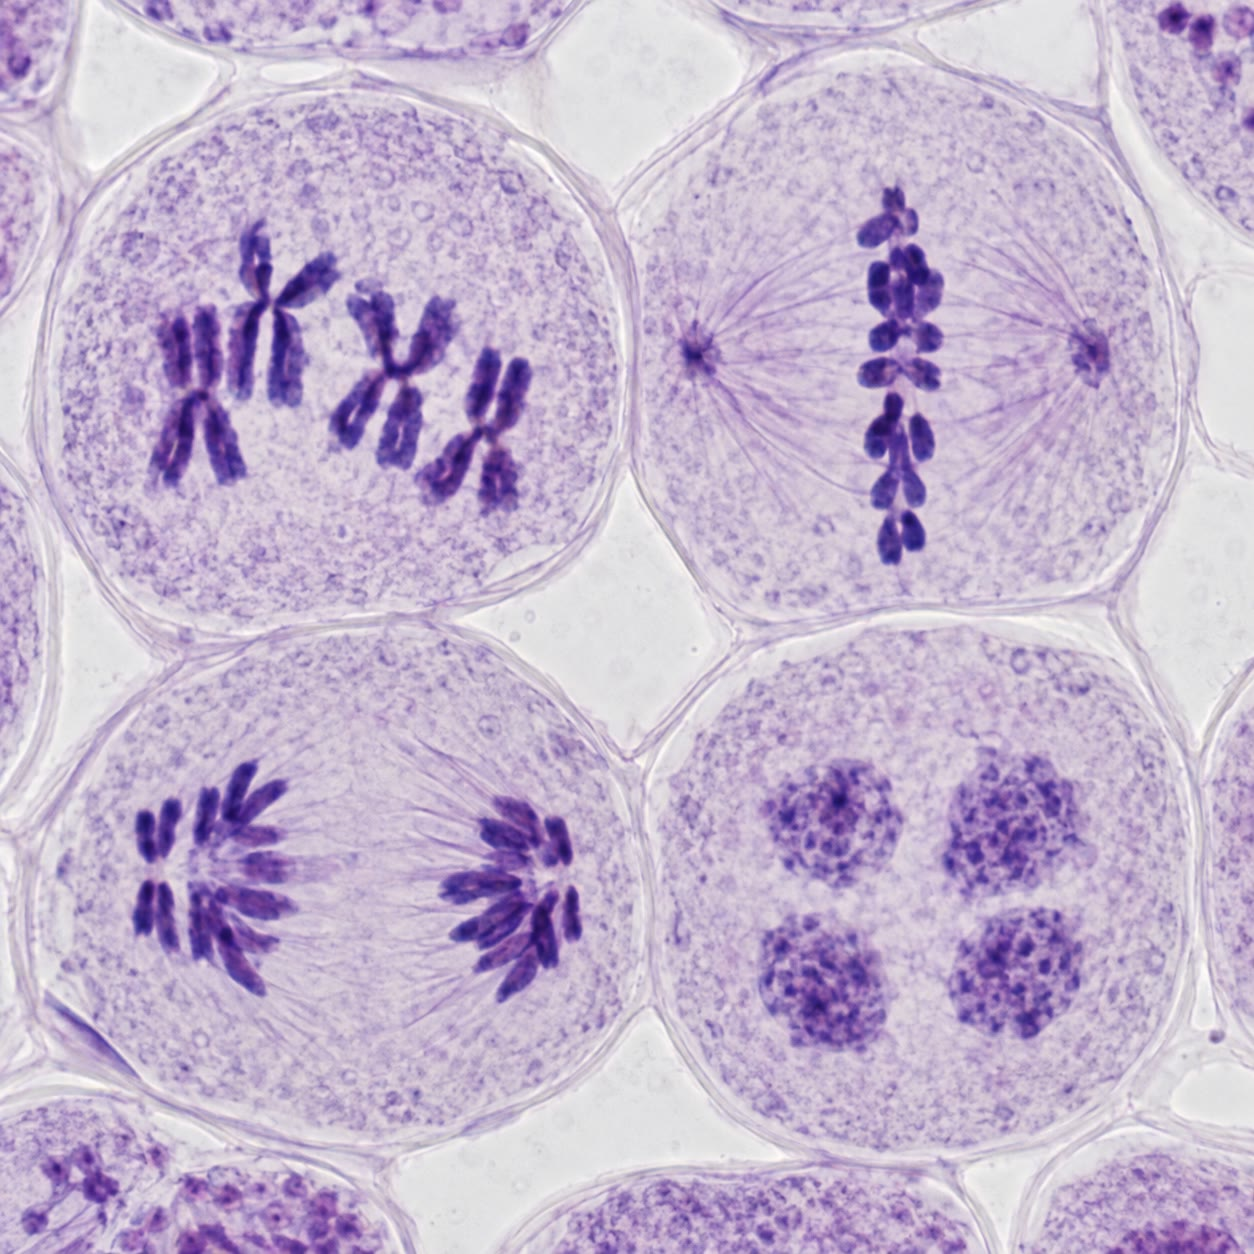
\includegraphics[width=0.5\linewidth]{images/book4/ai/b4-04-lily-meiosis.jpg}

{\small 百合花药中的\omterm{def:b2:meiosis-heredity:meiosis}{减数分裂}：前期 I 晚期的二价体、
中期 I 赤道板、后期 I，以及四分子的四个细胞核。}
\end{omfigure}

\begin{theorem}[减数分裂产生的混合程度]\label{thm:b2:meiosis-heredity:mixing}
\index{自由组合}\index{基因重组}
设生物具有 $n$ 对染色体，则中期 I 时二价体的随机取向
可产生 $2^n$ 种可能的母源与父源染色体组合，
出现于一个配子中——
人类中约为 $2^{23}$，约 840 万，而在一个
合子中为 $2^{2n}$。\omterm{prop:b2:meiosis-heredity:stages}{交叉互换}使之进一步倍增：每个二价体约有 $k$ 个\omterm{prop:b2:meiosis-heredity:stages}{交叉}，
各位置可变，因而不同配子的数目实际上不受限制，
同一个人的任何两个配子都不会相同。
\emph{重组}——\omterm{def:b2:meiosis-heredity:vocabulary}{等位基因}的新组合——
由二者共同产生：\omterm{thm:b2:meiosis-heredity:mixing}{自由组合}使整条染色体重新搭配，
\omterm{prop:b2:meiosis-heredity:stages}{交叉互换}则使一条染色体上的基因
在染色体内部重新搭配。
\end{theorem}
\begin{proof}
每个二价体的取向独立，各有两种结果，因此 $n$
个二价体给出 $2^n$ 种组合，且各组合等可能。双亲各
贡献一个这样的配子，故合子有 $2^n\times
2^n$ 种。在长为 $L$ 个碱基对的染色体上，若一次\omterm{prop:b2:meiosis-heredity:stages}{交叉}发生于不同位置，
每个二价体可产生数量级为 $L$ 的互异重组染色单体，
因此每条染色体上不同产物的数目按 $L^k$ 增长，
对于 $L \sim 10^8$ 而言，这一数目是天文数字。
\end{proof}
\begin{proof}[证据]
克赖顿与麦克林托克（1931）使用了玉米第 9 号染色体，其上带有
两个可见的细胞学标记（一端为染色体结，
另一端为易位片段），两者之间还有两个基因
（有色/无色籽粒，糯质/淀粉质胚乳）。在后代中，
凡具有重组\omterm{def:b2:meiosis-heredity:vocabulary}{等位基因}对的植株，也同时具有
重组的细胞学标记对——即有染色体结而无易位，
或相反情况，这证明\omterm{thm:b2:meiosis-heredity:mixing}{基因重组}是一种
染色体片段的物理交换。
\end{proof}

\begin{omfigure}
\begin{tikzpicture}[every node/.style={font=\scriptsize}]
  \foreach \dx/\lab/\ca/\cb/\gam in {0/{排列方式 1}/omDef/omThm/{配子 AB 和 ab}, 6.2/{排列方式 2}/omThm/omDef/{配子 Ab 和 aB}} {
    \begin{scope}[xshift=\dx cm]
      \draw[gray, dashed] (0,-1.1) -- (3.2,-1.1);
      \node[anchor=south] at (1.6,0.6) {\lab};
      % pair 1 (long): A above the plate, a below
      \draw[very thick, omDef] (0.7,-0.95) -- (0.7,-0.25); \node[omDef, anchor=south] at (0.7,-0.2) {A};
      \draw[very thick, omThm] (0.7,-1.25) -- (0.7,-1.95); \node[omThm, anchor=north] at (0.7,-2.0) {a};
      % pair 2 (short): B or b above depending on orientation
      \draw[very thick, \ca] (2.3,-0.85) -- (2.3,-0.35);
      \draw[very thick, \cb] (2.3,-1.35) -- (2.3,-1.85);
      \node[anchor=north] at (1.6,-2.4) {\gam};
    \end{scope}
  }
  \node[omDef, anchor=south] at (2.3,-0.3) {B}; \node[omThm, anchor=north] at (2.3,-1.9) {b};
  \node[omThm, anchor=south] at (8.5,-0.3) {b}; \node[omDef, anchor=north] at (8.5,-1.9) {B};
  \node[anchor=north, align=center] at (4.7,-3.0) {每种方向等可能：\\配子 AB、ab、Ab、aB 数目相等——独立分配};
\end{tikzpicture}

{\small 独立分配。对于两对染色体（一对为 A/a，另一对为 B/b），
中期 I 时二价体的两种可能取向
等可能出现，因此四种\omterm{def:b2:meiosis-heredity:vocabulary}{等位基因}组合
在配子中数目相等。}
\end{omfigure}

\section{孟德尔式分析}

\begin{definition}[杂交的术语]\label{def:b2:meiosis-heredity:vocabulary}
\index{等位基因}\index{基因型}\index{表型}\index{显性}\index{隐性}\index{纯合}\index{杂合}
\emph{基因}是染色体上的一段，其\emph{等位基因}为其
序列变体，\emph{基因座}为其位置。\omterm{def:b2:meiosis-heredity:meiosis}{二倍体}个体
在每个基因座上携带两个等位基因，其\emph{基因型}
为\emph{纯合}（$AA$、$aa$）或\emph{杂合}（$Aa$）。
\emph{表型}是可观测的性状。若某等位基因在杂合子中
即表现出其表型，则为\emph{显性}；
若仅在纯合子中才表现，则为\emph{隐性}。这一区分
是等位基因对与所观测性状的属性，而非单个等位基因的属性——
多数隐性等位基因是功能丧失型等位基因，
因只需一个有功能的拷贝即可发挥作用，故被掩盖。
\emph{纯系}能稳定遗传（纯合）；
\emph{测交}是让显性表型的个体与
隐性纯合子交配，使其后代
直接显示该个体配子中的等位基因。
\end{definition}

\begin{theorem}[孟德尔比率]\label{thm:b2:meiosis-heredity:mendel}
\index{孟德尔定律}\index{单杂交}\index{双杂交}
由于\omterm{def:b2:meiosis-heredity:vocabulary}{杂合}子 $Aa$ 的两个\omterm{def:b2:meiosis-heredity:vocabulary}{等位基因}
在\omterm{def:b2:meiosis-heredity:meiosis}{减数分裂}后期 I 分入数目相等的不同配子，一个\emph{\omterm{thm:b2:meiosis-heredity:mendel}{单杂交}}
$Aa \times Aa$ 得\omterm{def:b2:meiosis-heredity:vocabulary}{基因型} $\tfrac14 AA : \tfrac12 Aa :
\tfrac14 aa$，\omterm{def:b2:meiosis-heredity:vocabulary}{表型}为 $3 : 1$（$A$ 为\omterm{def:b2:meiosis-heredity:vocabulary}{显性}时）；测交
$Aa \times aa$ 得 $1 : 1$。由于位于不同
染色体上的\omterm{def:b2:meiosis-heredity:vocabulary}{等位基因}独立分配（中期 I），一个\emph{双\omterm{def:b2:meiosis-heredity:vocabulary}{杂合}子}
$AaBb$ 产生四种数目相等的配子，杂交
$AaBb \times AaBb$ 得\omterm{def:b2:meiosis-heredity:vocabulary}{表型} $9 : 3 : 3 : 1$，测交
$AaBb \times aabb$ 得 $1 : 1 : 1 : 1$。对于 $k$ 个独立
\omterm{def:b2:meiosis-heredity:vocabulary}{杂合}基因座，配子种类数为 $2^k$，且
\omterm{def:b2:meiosis-heredity:vocabulary}{表型}比为 $k$ 个 $3 : 1$ 之积。
\end{theorem}
\begin{proof}
分离：\omterm{def:b2:meiosis-heredity:vocabulary}{杂合}子的配子为 $\tfrac12 A$、
$\tfrac12 a$；随机受精时，合子\omterm{def:b2:meiosis-heredity:vocabulary}{基因型}即为
下列乘积 $(\tfrac12 A + \tfrac12 a)^2 = \tfrac14 AA + \tfrac12 Aa +
\tfrac14 aa$。独立性：$AaBb$ 的配子为 $(\tfrac12 A
+ \tfrac12 a)(\tfrac12 B + \tfrac12 b)$，共四种，每种 $\tfrac14$；
双\omterm{def:b2:meiosis-heredity:vocabulary}{杂合}子的\omterm{def:b2:meiosis-heredity:vocabulary}{表型}相乘为 $(\tfrac34 A\_ + \tfrac14 aa)
(\tfrac34 B\_ + \tfrac14 bb)$，得 $\tfrac{9}{16}, \tfrac{3}{16},
\tfrac{3}{16}, \tfrac{1}{16}$。每个因子对应一次独立的
分离，因此 $k$ 个基因座给出 $k$ 个因子之积。
\end{proof}
\begin{proof}[证据]
孟德尔（1866）以仅在一个性状上不同的纯系豌豆为材料进行杂交，
——种子为圆形或皱缩、子叶为黄色或绿色、花为紫色或
白花、茎为高或矮，以及另外三项——并在
每一情形中都得到一致的第一代，且第二代的
分离比接近 $3 : 1$：圆形 5474 粒对皱缩 1850 粒（$2.96 :
1$），黄色 6022 粒对绿色 2001 粒（$3.01 : 1$），紫花 705 株对白花 224 株
（$3.15 : 1$）。两性状杂交中，他得到 $315 : 108 : 101 :
32$（$9 : 3 : 3 : 1$），并通过种植第二代
证明\omterm{def:b2:meiosis-heredity:vocabulary}{显性}类别包含两种：三分之一为\omterm{def:b2:meiosis-heredity:vocabulary}{纯合}，
三分之二仍在分离。能解释这些比率的染色体
是在四十年后才被发现的。
\end{proof}

\begin{omfigure}
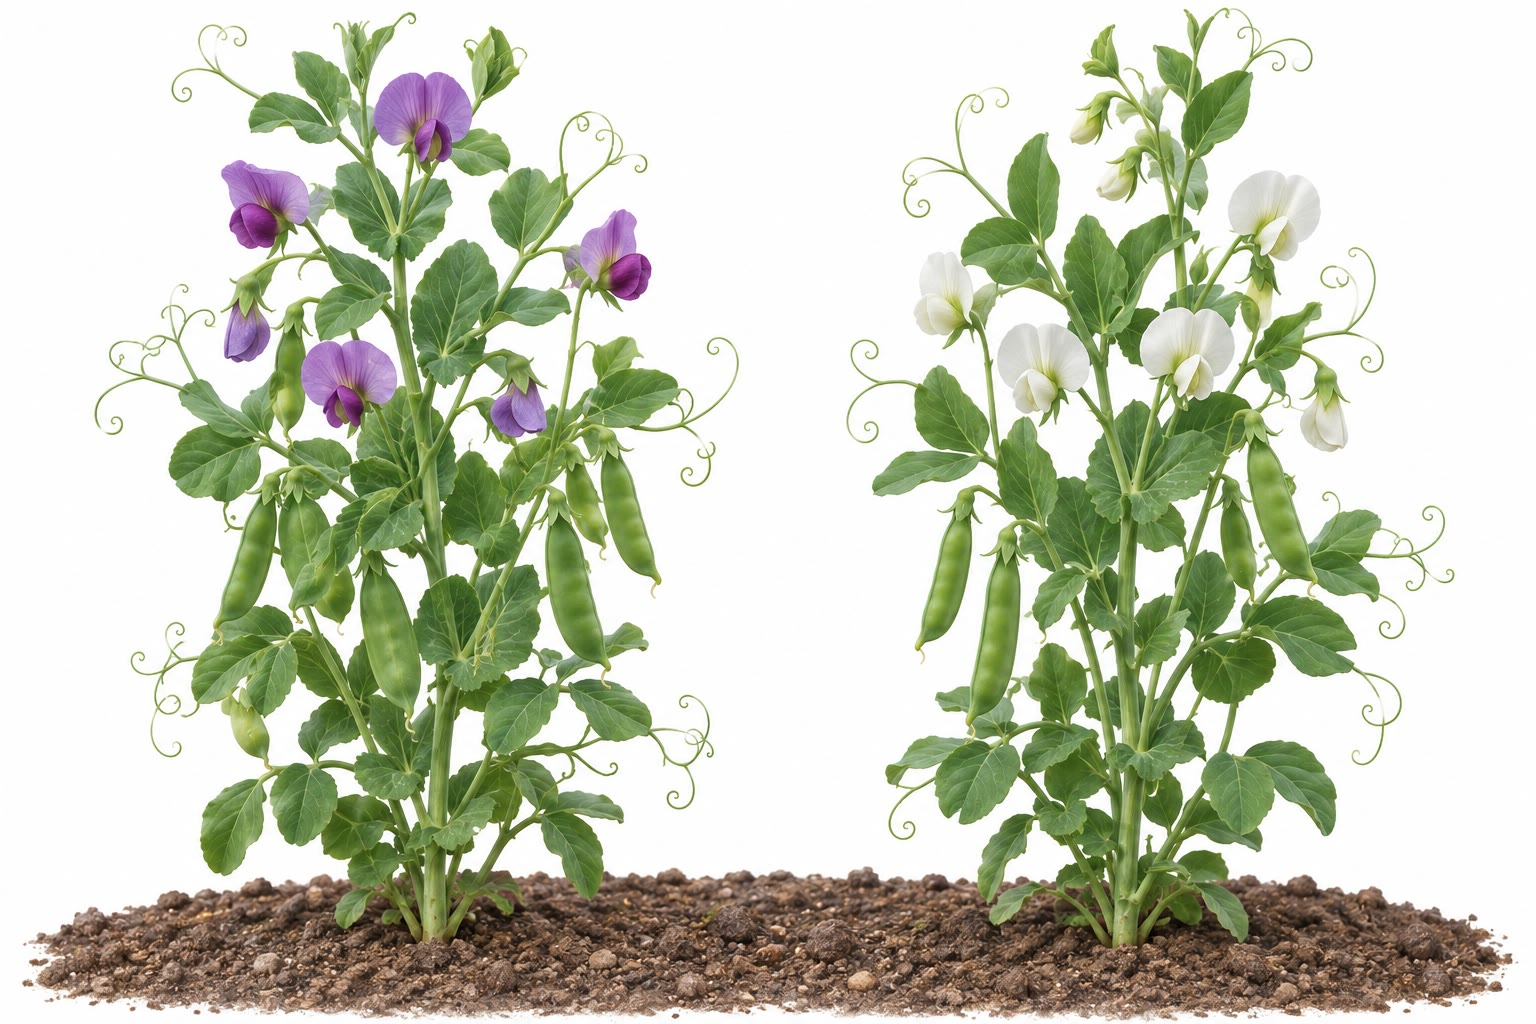
\includegraphics[width=0.58\linewidth]{images/book4/ai/b4-04-pea-flowers.jpg}

{\small 紫花与白花豌豆植株：孟德尔奠定遗传学所依据的
七对性状之一。紫花\omterm{def:b2:meiosis-heredity:vocabulary}{杂合}子自交，
后代中紫花与白花之比约为
三比一。}
\end{omfigure}

\begin{method}[用 $\chi^2$ 检验比率]\label{met:b2:meiosis-heredity:chisquare}
\index{卡方检验}
为判断观测计数 $O_i$ 是否符合某一假设比率：
\begin{enumerate}
  \item 由比率及
        总数计算期望计数 $E_i$。
  \item 计算 $\chi^2 = \sum_i (O_i - E_i)^2/E_i$。
  \item 计算自由度，即类别数
        减一。
  \item 与 \qty{5}{\%} 水平的临界值比较：
        自由度为 1 时为 $3.84$，为 2 时为 $5.99$，为 3 时为 $7.81$，
        为 4 时为 $9.49$。若 $\chi^2$ 小于该值，则数据
        与该比率相符；若大于该值，则拒绝该比率
——此偏差由偶然因素导致的情形，
        在不足二十分之一的实验中才会出现。
\end{enumerate}
对于孟德尔的花色数据，$705 : 224$ 对 $3 : 1$：$E = 696.75,
232.25$；$\chi^2 = 0.098 + 0.293 = 0.39 < 3.84$。（临界值所依据的
分布在数学丛书的
统计学中推导；此处将该表视为工具。）
\end{method}

\begin{proposition}[超越简单比率]\label{prop:b2:meiosis-heredity:extensions}
\index{不完全显性}\index{共显性}\index{上位性}\index{致死等位基因}
比率会改变，但机制不变，这发生于以下情形：\omterm{def:b2:meiosis-heredity:vocabulary}{等位基因}表现出
\emph{\omterm{prop:b2:meiosis-heredity:extensions}{不完全显性}}（红花 $\times$ 白花金鱼草杂交，
得粉花，第二代为 $1 : 2 : 1$）；\omterm{def:b2:meiosis-heredity:vocabulary}{等位基因}为
\emph{\omterm{prop:b2:meiosis-heredity:extensions}{共显性}}，两者都得到表达（$AB$ 型血中，
\omterm{def:b2:meiosis-heredity:vocabulary}{杂合}子 $I^AI^B$ 同时产生两种抗原；一个位点可能具有\emph{复\omterm{def:b2:meiosis-heredity:vocabulary}{等位基因}}（
$I^A$、$I^B$、$i$）；\omterm{def:b2:meiosis-heredity:vocabulary}{等位基因}在\omterm{def:b2:meiosis-heredity:vocabulary}{纯合}时为\emph{致死}
（黄色小鼠：黄色 $\times$ 黄色，后代为 $2$ 只黄色对
$1$ 只灰色，其中 $\tfrac14 YY$ 在胚胎期死亡）；两个基因在
同一条通路中起作用（\emph{\omterm{prop:b2:meiosis-heredity:extensions}{上位性}}：在 $9 : 3 : 3 : 1$ 的杂交中，双\omterm{def:b2:meiosis-heredity:vocabulary}{隐性}个体
与一种单\omterm{def:b2:meiosis-heredity:vocabulary}{隐性}个体的\omterm{def:b2:meiosis-heredity:vocabulary}{表型}可能无法区分，
得到 $9 : 3 : 4$，如白化小鼠；或两个\omterm{def:b2:meiosis-heredity:vocabulary}{显性}基因都需要才能形成\omterm{def:b2:meiosis-heredity:vocabulary}{表型}，
得到 $9 : 7$，如紫花香豌豆（需要两种酶来合成色素）；多个基因
各自对一个连续性状（身高、产量）作微小的累加贡献，
这正是\cref{ch:b2:population-genetics}中的数量遗传学。由比率反推机制，
是遗传学的
日常功夫。
\end{proposition}

\section{连锁与遗传图}

\begin{definition}[连锁与重组频率]\label{def:b2:meiosis-heredity:linkage}
\index{连锁}\index{重组频率}\index{厘摩}
位于同一条染色体上的两个基因称为\emph{连锁}基因：它们的\omterm{def:b2:meiosis-heredity:vocabulary}{等位基因}倾向于一起进入配子，
双\omterm{def:b2:meiosis-heredity:vocabulary}{杂合}子 $AB/ab$ 产生的\emph{亲本型}配子（$AB$、$ab$）多于
\emph{重组型}配子（$Ab$、$aB$）。重组型只有在
两位点之间发生交换时才会出现，
因此其频率 $r$——
在测交中直接计数——度量了距离：$r$
的取值从 0（完全连锁）到 $\tfrac12$（基因相距甚远，
或位于不同染色体上，以至于独立分配）。
\emph{图距}的单位为\emph{厘摩}（cM）：\qty{1}{cM}
对紧密连锁的基因而言即 \qty{1}{\%} 的重组；在人类中，
\qty{1}{cM} 约为一百万个碱基对。
连锁是基因沿染色体呈线性排列的第一个证据。
\end{definition}
\begin{proof}[证据]
摩尔根（1911）发现，果蝇的白眼基因与小翅基因
都位于 X 染色体上，二者并不独立分配：测交
得到 \qty{37}{\%} 的重组体，而非 \qty{50}{\%}；
其他基因对给出各不相同但可重复的百分比。斯特蒂文特（1913）
当时还是本科生，他意识到，若频率确实度量距离，
则它们应当可以相加：他由六个 X \omterm{def:b2:meiosis-heredity:linkage}{连锁}基因两两之间的频率
绘制出第一张遗传图，
并发现各距离在误差范围内沿一条直线确实可加。
\end{proof}

\begin{omfigure}
\begin{tikzpicture}[every node/.style={font=\scriptsize}]
  % bivalent with crossover between A and B
  \draw[very thick, omDef] (0,1.2) -- (2.0,1.2) -- (3.0,0.6) -- (5,0.6);
  \draw[very thick, omDef] (0,1.5) -- (5,1.5);
  \draw[very thick, omThm] (0,0.3) -- (2.0,0.3) -- (3.0,0.9) -- (5,0.9);
  \draw[very thick, omThm] (0,0) -- (5,0);
  \node[omDef, above] at (0.8,1.5) {A}; \node[omDef, above] at (4.3,1.5) {B};
  \node[omThm, below] at (0.8,0) {a}; \node[omThm, below] at (4.3,0) {b};
  \node[anchor=south, gray] at (2.5,1.85) {A、B 位点之间的交换};
  % products
  \draw[->, thick, gray] (5.4,0.75) -- (6.2,0.75);
  \node[anchor=west, align=left] at (6.4,1.45) {\textcolor{omDef}{A\,B} \quad 亲本型};
  \node[anchor=west, align=left] at (6.4,0.95) {\textcolor{omDef}{A}\,\textcolor{omThm}{b} \quad 重组型};
  \node[anchor=west, align=left] at (6.4,0.5) {\textcolor{omThm}{a}\,\textcolor{omDef}{B} \quad 重组型};
  \node[anchor=west, align=left] at (6.4,0.0) {\textcolor{omThm}{a\,b} \quad 亲本型};
  \node[anchor=west, align=left, text width=5.6cm] at (6.4,-0.9) {若在比例 $c$ 的减数分裂中两位点之间发生一次交换，则重组配子 $r = c/2$，因为四条染色单体中仅有两条发生互换};
\end{tikzpicture}

{\small 两个\omterm{def:b2:meiosis-heredity:linkage}{连锁}位点之间的重组。位于两位点之间的一次交换
在二价体中使四条染色单体中的两条交换\omterm{def:b2:meiosis-heredity:vocabulary}{等位基因}；
重组配子在测交中被计数，
其频率即度量了距离。}
\end{omfigure}

\begin{method}[定位两个连锁基因]\label{met:b2:meiosis-heredity:twopoint}
\begin{enumerate}
  \item 将两个纯系杂交得到双\omterm{def:b2:meiosis-heredity:vocabulary}{杂合}子，记下它同时获得了哪些\omterm{def:b2:meiosis-heredity:vocabulary}{等位基因}
        （其亲本组合，即\emph{偶联}
        $AB/ab$ 或\emph{相斥} $Ab/aB$）。
  \item 将其与双\omterm{def:b2:meiosis-heredity:vocabulary}{隐性}个体测交，并对后代分类：
        数量最多的两类为亲本型，
        数量最少的两类为重组型。
  \item $r = $ 重组体数 $/$ 总数；图距为 $100\,r$ cM。
  \item 先检验独立性：若四类数量相等
        （以 $\chi^2$ 检验比较 $1 : 1 : 1 : 1$），则两基因不\omterm{def:b2:meiosis-heredity:linkage}{连锁}。
\end{enumerate}
\end{method}

\begin{theorem}[霍尔丹作图函数]\label{thm:b2:meiosis-heredity:haldane}
\index{作图函数}
\omterm{def:b2:meiosis-heredity:linkage}{重组频率}会低估相距较远的基因之间的距离，
因为两者之间的两次交换会恢复亲本
组合。若交换沿染色体独立发生，
（无干涉）时，设 $d$ 为以摩根计的图距（
即每条染色单体上的期望交换次数），则重组率为
\[
r = \tfrac12\,\bigl(1 - e^{-2d}\bigr), \qquad d = -\tfrac12\ln(1 - 2r),
\]
因此 $r \approx d$（$d$ 较小时），而 $r \to \tfrac12$（$d$
增大时）；$r = 0.40$ 对应 \qty{80}{cM}，而 \qty{50}{cM}
对应 $r = 0.32$。真实染色体存在\emph{干涉}现象——一次交换
会使附近另一次交换的可能性降低——因而在短距离上，$r$
比霍尔丹的预测更接近 $d$。
\end{theorem}
\begin{proof}
设图距 $d$ 为该区间内每条染色单体上的
期望交换次数；由于每次交换都涉及四条染色单体中的两条，二价体整体
在该区间内的交换次数服从泊松分布，
均值为 $2d$，其不发生交换的概率为
$e^{-2d}$。若至少发生一次交换，则每次交换
独立地涉及某一给定染色单体的概率为
$\tfrac12$，因此某一给定染色单体被交换奇数次
（即为重组型）的概率恰好为 $\tfrac12$，
与交换次数无关。于是 $r = \tfrac12\,(1 -
e^{-2d})$；反解即得 $d$。当 $d$ 较小时，$r \approx d$；
当 $d \to \infty$ 时，$r \to \tfrac12$。
\end{proof}

\begin{omfigure}
\begin{tikzpicture}
\begin{axis}[
  width=0.72\linewidth, height=5.6cm,
  axis x line=bottom, axis y line=left,
  xmin=0, xmax=150, ymin=0, ymax=0.55,
  xlabel={图距 $d$（cM）}, ylabel={重组率 $r$},
  xlabel style={font=\small, at={(axis description cs:0.5,-0.13)}, anchor=north},
  ylabel style={font=\small},
  tick label style={font=\small}, xtick={0,50,100,150}, ytick={0,0.25,0.5},
  legend style={font=\scriptsize, at={(0.97,0.1)}, anchor=south east, draw=none},
  clip=false,
]
\addplot[very thick, omDef, domain=0:150, samples=80] {0.5*(1-exp(-2*x/100))};
\addlegendentry{霍尔丹：$r = \tfrac12(1 - e^{-2d})$}
\addplot[thick, dashed, gray, domain=0:50, samples=2] {x/100};
\addlegendentry{$r = d$（无双交换）}
\draw[dashed, gray] (axis cs:0,0.5) -- (axis cs:150,0.5);
\end{axis}
\end{tikzpicture}

{\small 重组率随图距的变化。近距基因
的重组率与其距离成正比；远距基因
的重组率无论相距多远都不超过 \qty{50}{\%}，
因为双交换会恢复亲本型组合。}
\end{omfigure}

\begin{method}[三点测交]\label{met:b2:meiosis-heredity:threepoint}
\index{三点测交}\index{干涉}
将三\omterm{def:b2:meiosis-heredity:vocabulary}{杂合}子 $ABC/abc$ 与 $abc/abc$ 测交，并对
八类子代进行分类。
\begin{enumerate}
  \item 数目最多的两类为亲本型，数目最少的两类
        为\emph{双交换}型。
  \item 在亲本类与双交换类之间发生改变的基因，
        即\emph{中间}基因：由此确定
        基因顺序。
  \item 对每对相邻基因，\omterm{def:b2:meiosis-heredity:linkage}{重组频率}为
        （该区间单交换数 + 双交换数）$/$
        总数；双交换使两个区间同时发生重组。
  \item 双交换的期望数 $= r_1 r_2 \times$ 总数；
        \emph{并发系数}为观察值/期望值，
        \emph{干涉}为 $1 -$ 并发系数。
\end{enumerate}
\end{method}

\begin{example}[三点测交实例]\label{ex:b2:meiosis-heredity:threepoint}
子代来自 $+++/abc \times abc/abc$：$+++$ 580，$abc$ 592，$++c$
45，$ab+$ 40，$+bc$ 89，$a++$ 94，$+b+$ 3，$a+c$ 5；总数 1448。
亲本型为 $+++$、$abc$；双交换型为 $+b+$、$a+c$；比较 $+++$ 与
$+b+$，发生改变的基因是 $b$，顺序为 $a$--$b$--$c$。$r_{ab} =
(89 + 94 + 3 + 5)/1448 = 0.132$; $r_{bc} = (45 + 40 + 3 + 5)/1448 =
0.064$；图距：$a$——\qty{13.2}{cM}——$b$——\qty{6.4}{cM}——
$c$。双交换的期望数 $0.132\times 0.064\times 1448 = 12.2$，
观察值为 8：并发系数 $0.65$，干涉 $0.35$。
\end{example}

\begin{omfigure}
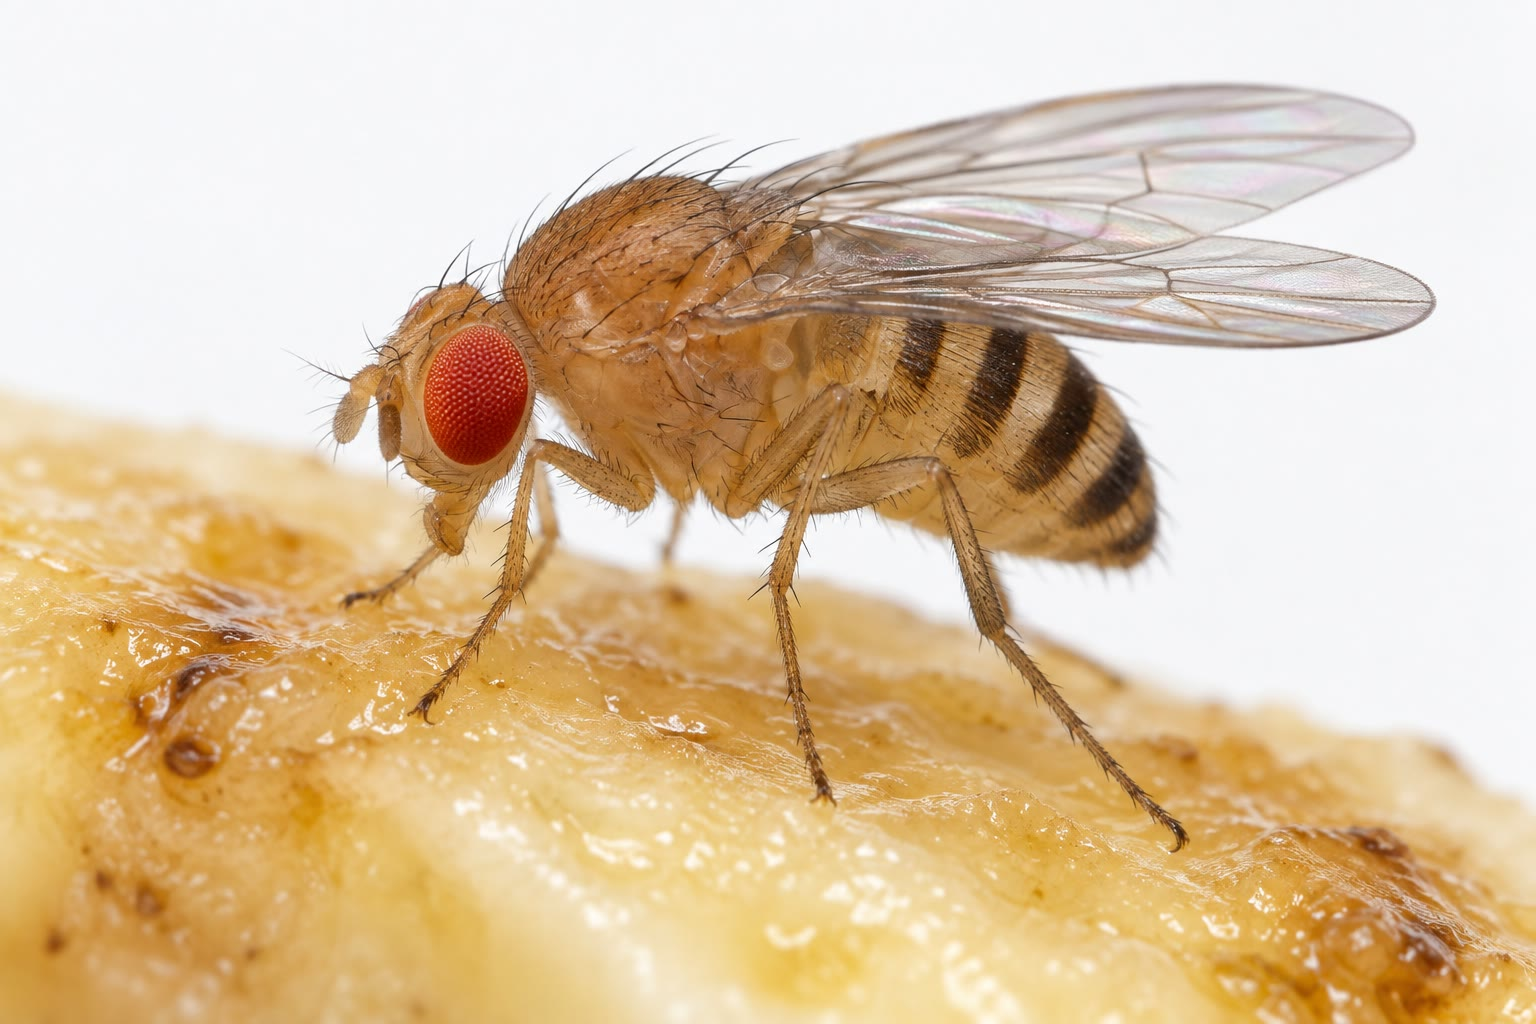
\includegraphics[width=0.5\linewidth]{images/book4/ai/b4-04-drosophila.jpg}

{\small \emph{Drosophila melanogaster}：每代两周，
子代数以百计，四对染色体，以及一个世纪积累的\omterm{def:b2:genome-diversification:mutation}{突变}体
——\omterm{def:b2:meiosis-heredity:linkage}{连锁}、图谱与伴性遗传正是在这种生物上
建立起来的。}
\end{omfigure}

\section{性染色体与细胞器}

\begin{proposition}[伴性遗传]\label{prop:b2:meiosis-heredity:sexlinked}
\index{X 连锁遗传}\index{性染色体}
在哺乳动物和蝇类中，雌性为 $XX$，雄性为 $XY$，其中 $Y$
染色体携带的基因很少，因此雄性每个 $X$ \omterm{def:b2:meiosis-heredity:linkage}{连锁}
基因只有一份（他是\emph{半合子}），表现出其所携带的
任何\omterm{def:b2:meiosis-heredity:vocabulary}{等位基因}，不论\omterm{def:b2:meiosis-heredity:vocabulary}{显性}或\omterm{def:b2:meiosis-heredity:vocabulary}{隐性}。由此可知正反交结果不同
（白眼雌 $\times$ 红眼雄得到白眼雄性子代和
红眼雌性子代；反交则全部为红眼）。一种\omterm{def:b2:meiosis-heredity:vocabulary}{隐性}的
$X$ \omterm{def:b2:meiosis-heredity:linkage}{连锁}性状（红绿色盲、血友病、杜氏
肌营养不良）多见于男性，由不发病的携带者母亲传递，
且从不由父亲传给儿子（儿子获得的是父亲的 $Y$）；
父亲则将其 $X$ 传给全部女儿。
鸟类、蝴蝶和部分爬行动物性别决定方式相反（$ZW$
为雌性，$ZZ$ 为雄性）；许多爬行动物由温度决定性别；而在
哺乳动物中，雌性每个细胞中的一条 $X$ 染色体在发育早期随机失活，
因此\omterm{def:b2:meiosis-heredity:vocabulary}{杂合}雌性是一种嵌合体（
玳瑁猫）。
\end{proposition}
\begin{proof}[证据]
摩尔根（1910）在数千只红眼果蝇中发现一只白眼雄蝇，
让其与红眼雌蝇杂交，子代全部为红眼；但
在下一代中，白眼性状只在雄性中重新出现，
且其中一半为白眼。让白眼雄蝇与其红眼女儿杂交，
子代两性均为白眼。这一结果恰与基因位于
X 染色体上的预期相符，因为雌性携带两份、雄性仅一份
——这是第一个被定位到某条染色体上的基因。
\end{proof}

\begin{omfigure}
\begin{tikzpicture}[every node/.style={font=\scriptsize}]
  % pedigree: X-linked recessive
  \draw[thick, fill=gray!70] (0,0) rectangle (0.5,0.5); % affected grandfather
  \draw[thick] (1.5,0.25) circle (0.25);
  \draw[thick] (0.5,0.25) -- (1.25,0.25);
  \draw[thick] (0.875,0.25) -- (0.875,-0.5);
  \draw[thick] (0.875,-0.5) -- (3.5,-0.5);
  % children of generation I
  \draw[thick] (0.875,-0.5) -- (0.875,-0.9); \draw[thick, fill=white] (0.875,-1.15) circle (0.25); \fill (0.875,-1.15) circle (0.08);
  \draw[thick] (2.2,-0.5) -- (2.2,-0.9); \draw[thick] (1.95,-1.4) rectangle (2.45,-0.9);
  \draw[thick] (3.5,-0.5) -- (3.5,-0.9); \draw[thick, fill=white] (3.5,-1.15) circle (0.25); \fill (3.5,-1.15) circle (0.08);
  % carrier daughter marries
  \draw[thick] (-0.3,-1.15) -- (0.625,-1.15); \draw[thick] (-0.55,-1.4) rectangle (-0.05,-0.9);
  \draw[thick] (0.15,-1.15) -- (0.15,-1.9); \draw[thick] (-1.2,-1.9) -- (1.5,-1.9);
  \draw[thick] (-1.2,-1.9) -- (-1.2,-2.3); \draw[thick, fill=gray!70] (-1.45,-2.8) rectangle (-0.95,-2.3);
  \draw[thick] (-0.3,-1.9) -- (-0.3,-2.3); \draw[thick] (-0.55,-2.8) rectangle (-0.05,-2.3);
  \draw[thick] (0.6,-1.9) -- (0.6,-2.3); \draw[thick, fill=white] (0.6,-2.55) circle (0.25); \fill (0.6,-2.55) circle (0.08);
  \draw[thick] (1.5,-1.9) -- (1.5,-2.3); \draw[thick, fill=white] (1.5,-2.55) circle (0.25);
  \node[anchor=east] at (-1.8,0.25) {I};
  \node[anchor=east] at (-1.8,-1.15) {II};
  \node[anchor=east] at (-1.8,-2.55) {III};
  % legend
  \node[anchor=west, align=left] at (5,-0.4) {$\square$ 男 \quad $\bigcirc$ 女};
  \draw[thick, fill=gray!70] (5.05,-1.25) rectangle (5.45,-0.85); \node[anchor=west] at (5.6,-1.05) {患病};
  \draw[thick] (5.25,-1.85) circle (0.2); \fill (5.25,-1.85) circle (0.07); \node[anchor=west] at (5.6,-1.85) {携带者（杂合子）};
  \node[anchor=north west, align=left, text width=6.2cm] at (5,-2.3) {X 连锁隐性：患病男性的子女均不患病，其所有女儿都携带该等位基因，而她们的儿子有一半患病——该性状隔代出现，在外孙中重新出现};
\end{tikzpicture}

{\small 一张 X \omterm{def:b2:meiosis-heredity:linkage}{连锁}\omterm{def:b2:meiosis-heredity:vocabulary}{隐性}性状（如血友病）的\omterm{met:b2:meiosis-heredity:pedigree}{系谱图}：
无父传子，携带者女儿，
患病的外孙。}
\end{omfigure}

\begin{method}[读懂系谱图]\label{met:b2:meiosis-heredity:pedigree}
\index{系谱图}
\begin{enumerate}
  \item 双亲\omterm{def:b2:meiosis-heredity:vocabulary}{表型}正常而生下患病子女：该性状为\omterm{def:b2:meiosis-heredity:vocabulary}{隐性}
        （双亲均为\omterm{def:b2:meiosis-heredity:vocabulary}{杂合}子）。
  \item 患病子女必有患病的亲代，
        该性状每一代都出现：为\omterm{def:b2:meiosis-heredity:vocabulary}{显性}。
  \item 患病者多为男性，经\omterm{def:b2:meiosis-heredity:vocabulary}{表型}正常的母亲传递，
        从不由父亲传给儿子：X \omterm{def:b2:meiosis-heredity:linkage}{连锁}\omterm{def:b2:meiosis-heredity:vocabulary}{隐性}。
  \item 患病父亲的所有女儿均患病，
        且儿子均不患病：X \omterm{def:b2:meiosis-heredity:linkage}{连锁}\omterm{def:b2:meiosis-heredity:vocabulary}{显性}。
  \item 由母亲传给全部子女，
        从不由父亲传递：\omterm{def:b2:meiosis-heredity:extranuclear}{线粒体遗传}。
  \item 再由推出的\omterm{def:b2:meiosis-heredity:vocabulary}{基因型}计算概率：
        携带者 $\times$ 正常人婚配时，每次生育患病儿子的概率为 $\tfrac14$
        （$\tfrac12$ 为男孩 $\times$ $\tfrac12$
        获得该\omterm{def:b2:meiosis-heredity:vocabulary}{等位基因}）。
\end{enumerate}
\end{method}

\begin{definition}[核外遗传]\label{def:b2:meiosis-heredity:extranuclear}
\index{母系遗传}\index{线粒体遗传}
线粒体和叶绿体各自携带一套小型基因组，
每个细胞器中有多份拷贝，每个细胞中有多个细胞器，它们
几乎完全来自卵细胞，精子只提供细胞核，
别无其他。因此，它们的基因\emph{母系遗传
}，不呈现分离比：母亲将该性状传给
全部子女，父亲则一个也不传。人类线粒体疾病
（呼吸链缺陷，影响肌肉和神经）
遵循这一模式，某些植物的斑驳现象亦然：
含有正常与\omterm{def:b2:genome-diversification:mutation}{突变}叶绿体的母细胞，
将它们随机分配到子细胞中，产生绿色、白色和混合的扇形区域。
由于它们从不重组，线粒体序列
可追溯母系谱系的历史——正是
\cref{ch:b2:phylogenetic-trees}所用的工具。
\end{definition}

\begin{proposition}[四分体分析]\label{prop:b2:meiosis-heredity:tetrads}
\index{四分体分析}\index{有序四分体}
在某些真菌（\emph{Neurospora}、\emph{Sordaria}）中，一次\omterm{def:b2:meiosis-heredity:meiosis}{减数分裂}的四个产物
留在一个囊（即\emph{子囊}）中，并按顺序排列：再经一次有丝分裂，
得到八个孢子，其排列顺序记录了两次分裂。
对于\omterm{def:b2:meiosis-heredity:vocabulary}{杂合}子 $A/a$，
子囊呈 $4 : 4$（\emph{第一次分裂分离}）型时，基因与其着丝粒之间无交换——
\omterm{def:b2:meiosis-heredity:vocabulary}{等位基因}在减数第一次分裂后期分开；子囊呈
$2 : 2 : 2 : 2$ 或 $2 : 4 : 2$（\emph{第二次分裂分离}）型时，存在交换，
\omterm{def:b2:meiosis-heredity:vocabulary}{等位基因}仅在减数第二次分裂后期才分开。
从基因到着丝粒的距离，等于第二次分裂分离子囊百分比的一半，
因为一次交换只重组四条染色单体中的两条。
四分体还直接表明，重组是相互的：
每条重组染色单体都有互补的
伙伴位于同一子囊中。
\end{proposition}

\begin{omfigure}
\begin{tikzpicture}[every node/.style={font=\scriptsize}]
  \foreach \dx/\pat/\lab in {0/{omDef,omDef,omDef,omDef,omThm,omThm,omThm,omThm}/{$4:4$，无交换：\\第一次分裂分离}, 4.5/{omDef,omDef,omThm,omThm,omDef,omDef,omThm,omThm}/{$2:2:2:2$，基因与 \\着丝粒之间发生交换}, 9/{omDef,omDef,omThm,omThm,omThm,omThm,omDef,omDef}/{$2:4:2$，发生交换：\\第二次分裂分离}} {
    \begin{scope}[xshift=\dx cm]
      \draw[thick, rounded corners=6pt] (0,0) rectangle (0.8,4.2);
      \foreach \c [count=\i] in \pat { \fill[\c] (0.4,4.2-0.5*\i+0.02) circle (0.2); }
      \node[below, align=center] at (0.4,-0.1) {\lab};
    \end{scope}
  }
  \node[anchor=west, align=left, text width=2.6cm] at (12.4,3.2) {\emph{Sordaria} 的有序子囊；蓝色和红色孢子携带两种等位基因};
\end{tikzpicture}

{\small \omterm{prop:b2:meiosis-heredity:tetrads}{有序四分体}。基因与着丝粒之间无交换时，
\omterm{def:b2:meiosis-heredity:vocabulary}{等位基因}在第一次分裂时分开，八个孢子读作
$4 : 4$；有交换时，\omterm{def:b2:meiosis-heredity:vocabulary}{等位基因}在第二次分裂时分开，
子囊读作 $2 : 2 : 2 : 2$ 或 $2 : 4 : 2$。}
\end{omfigure}

\section{练习}

\begin{exercise}[$\star$]\label{exo:b2:meiosis-heredity:1}
列出有丝分裂与\omterm{def:b2:meiosis-heredity:meiosis}{减数分裂}之间的四点区别
（分裂次数、配对、产物、产物的遗传同一性）。
\end{exercise}

\begin{exercise}[$\star$]\label{exo:b2:meiosis-heredity:2}
一个人仅靠独立分配，
能产生多少种染色体组成不同的配子？果蝇（$n = 4$）呢？豌豆（$n =
7$）呢？
\end{exercise}

\begin{exercise}[$\star$]\label{exo:b2:meiosis-heredity:3}
豌豆中，高茎（$T$）对矮茎为\omterm{def:b2:meiosis-heredity:vocabulary}{显性}。给出
$Tt \times Tt$ 与 $Tt \times tt$ 的\omterm{def:b2:meiosis-heredity:vocabulary}{表型}比和\omterm{def:b2:meiosis-heredity:vocabulary}{基因型}比。如何
判断一株高茎植物是 $TT$ 还是 $Tt$？
\end{exercise}

\begin{exercise}[$\star$]\label{exo:b2:meiosis-heredity:4}
定义\omterm{def:b2:meiosis-heredity:linkage}{连锁}、重组率和\omterm{def:b2:meiosis-heredity:linkage}{厘摩}。为什么
位于同一染色体上的两个基因，仍可表现得如同
独立分配一样？
\end{exercise}

\begin{exercise}[$\star\star$]\label{exo:b2:meiosis-heredity:5}
孟德尔的双因子杂交得到 $315$ 株圆粒黄色、$108$ 株圆粒绿色、
$101$ 株皱粒黄色、$32$ 株皱粒绿色。检验 $9 : 3 : 3 :
1$ 的假设，用 $\chi^2$ 检验（自由度为 3，临界值
$7.81$）。
\end{exercise}

\begin{exercise}[$\star\star$]\label{exo:b2:meiosis-heredity:6}
双\omterm{def:b2:meiosis-heredity:vocabulary}{杂合}子 $AB/ab$ 测交得到 $412$ 个 $AB$、$388$ 个 $ab$、$103$
个 $Ab$、$97$ 个 $aB$。这两个基因是否\omterm{def:b2:meiosis-heredity:linkage}{连锁}？计算重组率
和图距；双\omterm{def:b2:meiosis-heredity:vocabulary}{杂合}子 $Ab/aB$ 的结果会是什么？
\end{exercise}

\begin{exercise}[$\star\star$]\label{exo:b2:meiosis-heredity:7}
利用霍尔丹函数，将 $r = 0.20$ 和 $r = 0.45$ 换算为图距，
并将 \qty{30}{cM} 和 \qty{100}{cM} 换算为重组率。
讨论哪些换算在实践中更有意义。
\end{exercise}

\begin{exercise}[$\star\star$]\label{exo:b2:meiosis-heredity:8}
在\emph{Drosophila}中，白眼（$w$）为 X \omterm{def:b2:meiosis-heredity:linkage}{连锁}\omterm{def:b2:meiosis-heredity:vocabulary}{隐性}性状。求下列杂交子代的性别与\omterm{def:b2:meiosis-heredity:vocabulary}{表型}：
(a) 白眼雌性 $\times$ 红眼雄性；(b) 红眼\omterm{def:b2:meiosis-heredity:vocabulary}{杂合}雌性 $\times$ 白眼雄性；
(c) 为 (a) 中子代雌性
与其兄弟的杂交。
\end{exercise}

\begin{exercise}[$\star\star$]\label{exo:b2:meiosis-heredity:9}
两个白花香豌豆纯系杂交，所得子代全部为
紫花，子代自交得 $9$ 紫花：$7$ 白花。
用两对基因加以解释，求两个亲本纯系的\omterm{def:b2:meiosis-heredity:vocabulary}{基因型}，
并预测紫花杂种测交的结果。
\end{exercise}

\begin{exercise}[$\star\star\star$]\label{exo:b2:meiosis-heredity:10}
\omterm{met:b2:meiosis-heredity:threepoint}{三点测交}的结果为：$+++$ 480，$abc$ 470，$+bc$ 11，
$a++$ 9，$++c$ 118，$ab+$ 112，$+b+$ 1，$a+c$ 1（总数 1202）。求
基因顺序、两段图距、并发系数
与干涉。
\end{exercise}

\begin{exercise}[$\star\star\star$]\label{exo:b2:meiosis-heredity:11}
在\emph{Sordaria}中，黑色孢子品系与
棕色孢子品系杂交，得到 $700$ 个 $4 : 4$ 型子囊，以及 $300$ 个
$2 : 2 : 2 : 2$ 型或 $2 : 4 : 2$ 型子囊。计算
孢子颜色基因到其着丝粒的距离，并解释为何需要
因子二分之一。画出一次\omterm{def:b2:meiosis-heredity:meiosis}{减数分裂}产生
$2 : 4 : 2$ 型时的染色单体。
\end{exercise}

\begin{exercise}[$\star\star\star$]\label{exo:b2:meiosis-heredity:12}
某女性的外祖父患血友病，家族中
其他人均未患病。她是携带者的概率是多少？
若已知她生有两个健康的儿子，此概率又为多少？请写出
推理过程。
\end{exercise}

\section{问题：果蝇室中的杂交}

\begin{problem}[{周末问题——对\emph{Drosophila}杂交的分析，由单因子比例
推至三点图谱，并计算一个人类系谱，
最后得到三个 X \omterm{def:b2:meiosis-heredity:linkage}{连锁}基因的图谱，
及其干涉}]
\label{pb:b2:meiosis-heredity:1}
残翅（$vg$）和黑檀体（$e$）为\omterm{def:b2:meiosis-heredity:vocabulary}{隐性}，位于
不同的常染色体上；黑体（$b$）与 $vg$ 为\omterm{def:b2:meiosis-heredity:vocabulary}{隐性}，两者均
位于 2 号染色体上；黄体（$y$）、白眼（$w$）和小翅（$m$）为\omterm{def:b2:meiosis-heredity:vocabulary}{隐性}，
且为 X \omterm{def:b2:meiosis-heredity:linkage}{连锁}。$\chi^2$ 在 \qty{5}{\%} 水平下的临界值为：
$3.84$（1 个自由度），$7.81$（3 个自由度）。

\medskip
\noindent\textbf{第一部分——两对常染色体基因。}
将\omterm{def:b2:meiosis-heredity:vocabulary}{纯合}残翅果蝇与\omterm{def:b2:meiosis-heredity:vocabulary}{纯合}黑檀体果蝇杂交，$F_1$
全部为野生型；统计 $1600$ 只 $F_2$ 果蝇：$892$ 只野生型，$309$
只残翅，$296$ 只黑檀体，$103$ 只残翅黑檀体。
\begin{enumerate}
  \item 求亲本、$F_1$ 及
        $F_1$ 配子的\omterm{def:b2:meiosis-heredity:vocabulary}{基因型}。
  \item 计算独立分配下的期望数。
  \item 计算 $\chi^2$ 并作出结论。
  \item 野生型 $F_2$ 果蝇中，
        两个基因座均为\omterm{def:b2:meiosis-heredity:vocabulary}{纯合}的比例是多少？
  \item 将 $F_1$ 与残翅黑檀体果蝇测交：预测
        四类\omterm{def:b2:meiosis-heredity:vocabulary}{表型}及其比例。
  \item 在 \qty{29}{\celsius} 下饲养的黑檀体果蝇，
        颜色比在 \qty{18}{\celsius} 下更浅。这说明
        \omterm{def:b2:meiosis-heredity:vocabulary}{基因型}与\omterm{def:b2:meiosis-heredity:vocabulary}{表型}之间的关系如何？
\end{enumerate}

\medskip
\noindent\textbf{第二部分——两个\omterm{def:b2:meiosis-heredity:linkage}{连锁}基因。}
将\omterm{def:b2:meiosis-heredity:vocabulary}{纯合}黑体果蝇与\omterm{def:b2:meiosis-heredity:vocabulary}{纯合}残翅果蝇杂交，$F_1$
雌性与黑体残翅雄性测交：$965$ 只黑体，
$944$ 只残翅，$206$ 只黑体残翅，$185$ 只野生型。
\begin{enumerate}[resume]
  \item 写出 $F_1$ 的\omterm{def:b2:meiosis-heredity:vocabulary}{基因型}，标明哪些\omterm{def:b2:meiosis-heredity:vocabulary}{等位基因}位于
        同一条染色体上。
  \item 指出亲本型与重组型，并解释为何此处的
        野生型属于\emph{重组型}。
  \item 计算 $r$ 及图距。
  \item 用霍尔丹函数校正。
  \item 若以 $F_1$ \emph{雄性}进行同样的测交，仅得到两类，
        即黑体与残翅，且数目相等。这说明雄果蝇
        \omterm{def:b2:meiosis-heredity:meiosis}{减数分裂}有何特点？
  \item 若 $F_1$ 雌性来自黑体残翅 $\times$ 野生型的杂交，
        则预测各类\omterm{def:b2:meiosis-heredity:vocabulary}{表型}及其比例。
\end{enumerate}

\medskip
\noindent\textbf{第三部分——一个人类系谱。}
血友病 A 为 X \omterm{def:b2:meiosis-heredity:linkage}{连锁}\omterm{def:b2:meiosis-heredity:vocabulary}{隐性}遗传。一名患血友病的男子有一个女儿，
该女儿与一名未患病的男子结婚。
\begin{enumerate}[resume]
  \item 该女儿的\omterm{def:b2:meiosis-heredity:vocabulary}{基因型}是什么？为何可以确定？
  \item 她的第一个孩子是患病儿子的概率。
  \item 她的女儿为携带者的概率。
  \item 在她的三个孩子中，无一人
        患病的概率。
  \item 解释为何该病从不由父亲传给儿子，
        以及女性如何会患病。
  \item 该患病男子的妹妹有两个健康的儿子；其母亲
        （即该男子的母亲）为携带者。求该妹妹为携带者的概率，
        分别在未计入其儿子之前与计入之后的
        概率。
\end{enumerate}

\medskip
\noindent\textbf{第四部分——三个 X \omterm{def:b2:meiosis-heredity:linkage}{连锁}基因。}
将雌果蝇 $y\,w\,m/+\,+\,+$ 与 $y\,w\,m$ 雄果蝇杂交，其 $2000$ 只
儿子经统计：$+++$ 853，$ywm$ 833，$y++$ 24，$+wm$ 26，$yw+$ 128，
$++m$ 132，$+w+$ 2，$y+m$ 2。
\begin{enumerate}[resume]
  \item 为何这些儿子可直接统计，而无需测交？
  \item 指出亲本型与双交换型，
        并推断基因顺序。
  \item 计算两个重组率并画出图谱。
  \item 计算双交换的期望数、
        并发系数和干涉。
  \item 直接由数据计算两个外侧基因之间的
        重组率，并解释为何它
        小于两段图距之和。
  \item 该杂交的女儿会呈现怎样的\omterm{def:b2:meiosis-heredity:vocabulary}{表型}？为何
        她们对作图没有用处？
  \item 给出结论：三个基因的图谱及
        其干涉。
\end{enumerate}
\end{problem}
